\documentclass[12pt,a4paper]{article}
\usepackage[utf8]{inputenc}
\usepackage{graphicx}
\usepackage{hyperref}
\usepackage{xcolor}
\usepackage{geometry}
\usepackage{setspace}
\usepackage{caption}
\usepackage{float}
\usepackage{booktabs}

\geometry{margin=1in}
\setstretch{1.3}

\begin{document}

%------------------- TITLE PAGE -------------------%
\begin{titlepage}
\centering
{\LARGE \textbf{Report: Big Data Stock Price Analysis}}\\[2cm]
{\large Analysis of VNStock Data Using Hadoop \& Spark}\\[1cm]
{\large \textbf{Data Source: VNStock (2015–2025)}}\\[2cm]
\textbf{Author:} Trinh Tuan Ngoc Bao\\[0.5cm]
\textbf{Institution:} University of Engineering and Technology – Big Data\\[0.5cm]
\textbf{Date:} \today
\end{titlepage}

\tableofcontents
\newpage

%------------------- ABSTRACT -------------------%
\begin{abstract}
This report presents the development of a distributed Big Data analytics system for analyzing Vietnamese stock market data from VNStock.
The project demonstrates an end-to-end data pipeline including data collection, storage, preprocessing, and distributed analysis on a Docker-based Hadoop–Spark cluster.
The system efficiently handles thousands of stock records and performs analytical tasks such as price trend tracking and growth rate comparison across major Vietnamese bank stocks.
\end{abstract}

%------------------- INTRODUCTION -------------------%
\section{Introduction}

The Vietnamese stock market has expanded rapidly in both transaction volume and market capitalization.  
Consequently, traditional data processing tools struggle to handle the growing scale and velocity of market data.  

This project builds a simulated Big Data environment for analyzing stock prices using VNStock as the primary data source.  
It integrates the \textbf{Hadoop Distributed File System (HDFS)} for scalable storage and \textbf{Apache Spark} for distributed computation.  
The approach demonstrates the advantages of Big Data technologies in managing and analyzing financial time-series data efficiently.

%------------------- THEORETICAL BACKGROUND -------------------%
\section{Theoretical Background}

\subsection{Big Data Systems}
Big Data refers to datasets with massive volume, variety, and velocity, which require distributed systems for efficient storage and analysis.  
Frameworks such as Hadoop and Spark enable horizontal scalability and high processing speed.

\subsection{Hadoop and HDFS}
Hadoop provides distributed data storage through HDFS, allowing large files to be partitioned across multiple DataNodes.  
A central NameNode manages metadata, ensuring fault tolerance and high availability.

\subsection{Apache Spark}
Apache Spark is an in-memory data processing engine designed for large-scale distributed computation.  
It performs transformations and aggregations much faster than traditional MapReduce, making it ideal for iterative analytics tasks such as stock trend analysis.

\subsection{Stock Data Characteristics}
Stock market data are a form of time-series data — values recorded sequentially over time.  
They are highly dynamic and influenced by numerous market factors, requiring efficient systems for continuous collection and processing.

%------------------- SYSTEM DESIGN -------------------%
\section{System Design and Implementation}

\subsection{System Architecture}
The system was deployed using Docker Compose and consists of:

\begin{itemize}
    \item \textbf{HDFS Cluster:} One NameNode and four DataNodes to store distributed data.
    \item \textbf{Spark Cluster:} One Spark Master and four Spark Workers for distributed computation.
    \item \textbf{Jupyter Notebook:} An interactive interface for accessing the Spark cluster.
\end{itemize}

\begin{figure}[H]
    \centering
    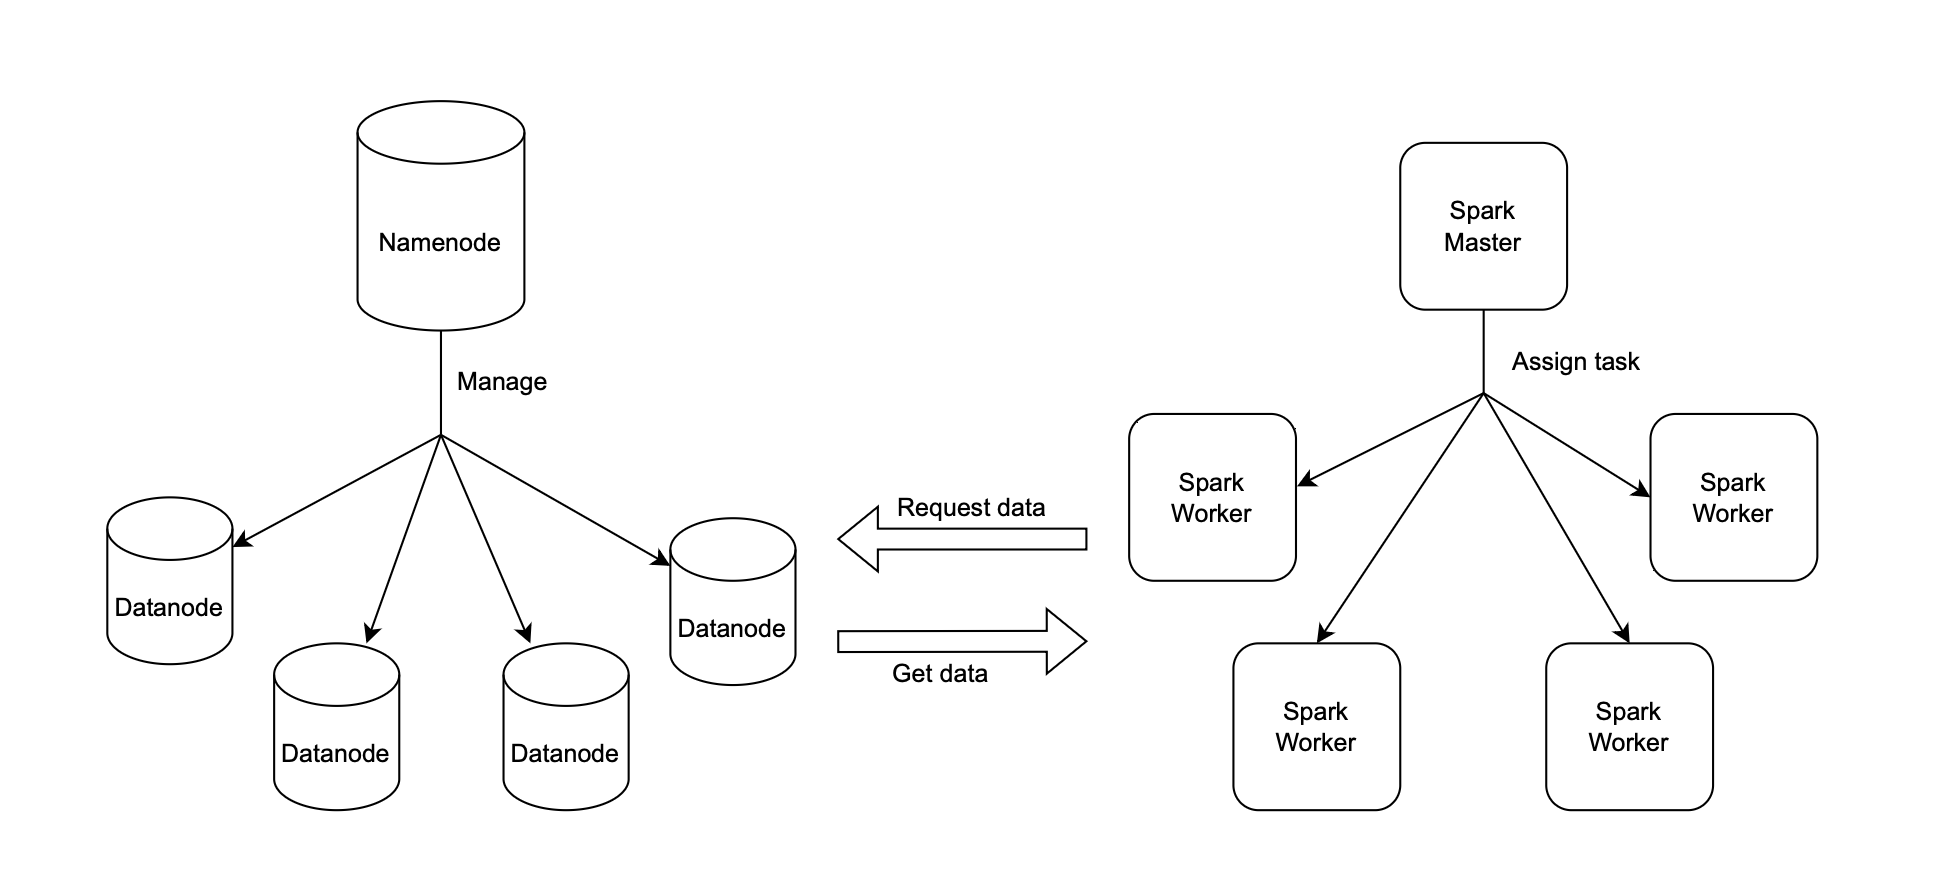
\includegraphics[width=0.9\textwidth]{architecture.png}
    \caption{System architecture integrating Hadoop and Spark clusters.}
\end{figure}

\subsection{Cluster Setup}
Each node is deployed as a Docker container using the following images:

\begin{itemize}
    \item \texttt{bde2020/hadoop-namenode:2.0.0-hadoop3.2.1-java8}
    \item \texttt{bde2020/hadoop-datanode:2.0.0-hadoop3.2.1-java8}
    \item \texttt{spark:3.5.0} (for both Master and Workers)
    \item \texttt{jupyter/pyspark-notebook:latest}
\end{itemize}

\begin{figure}[H]
    \centering
    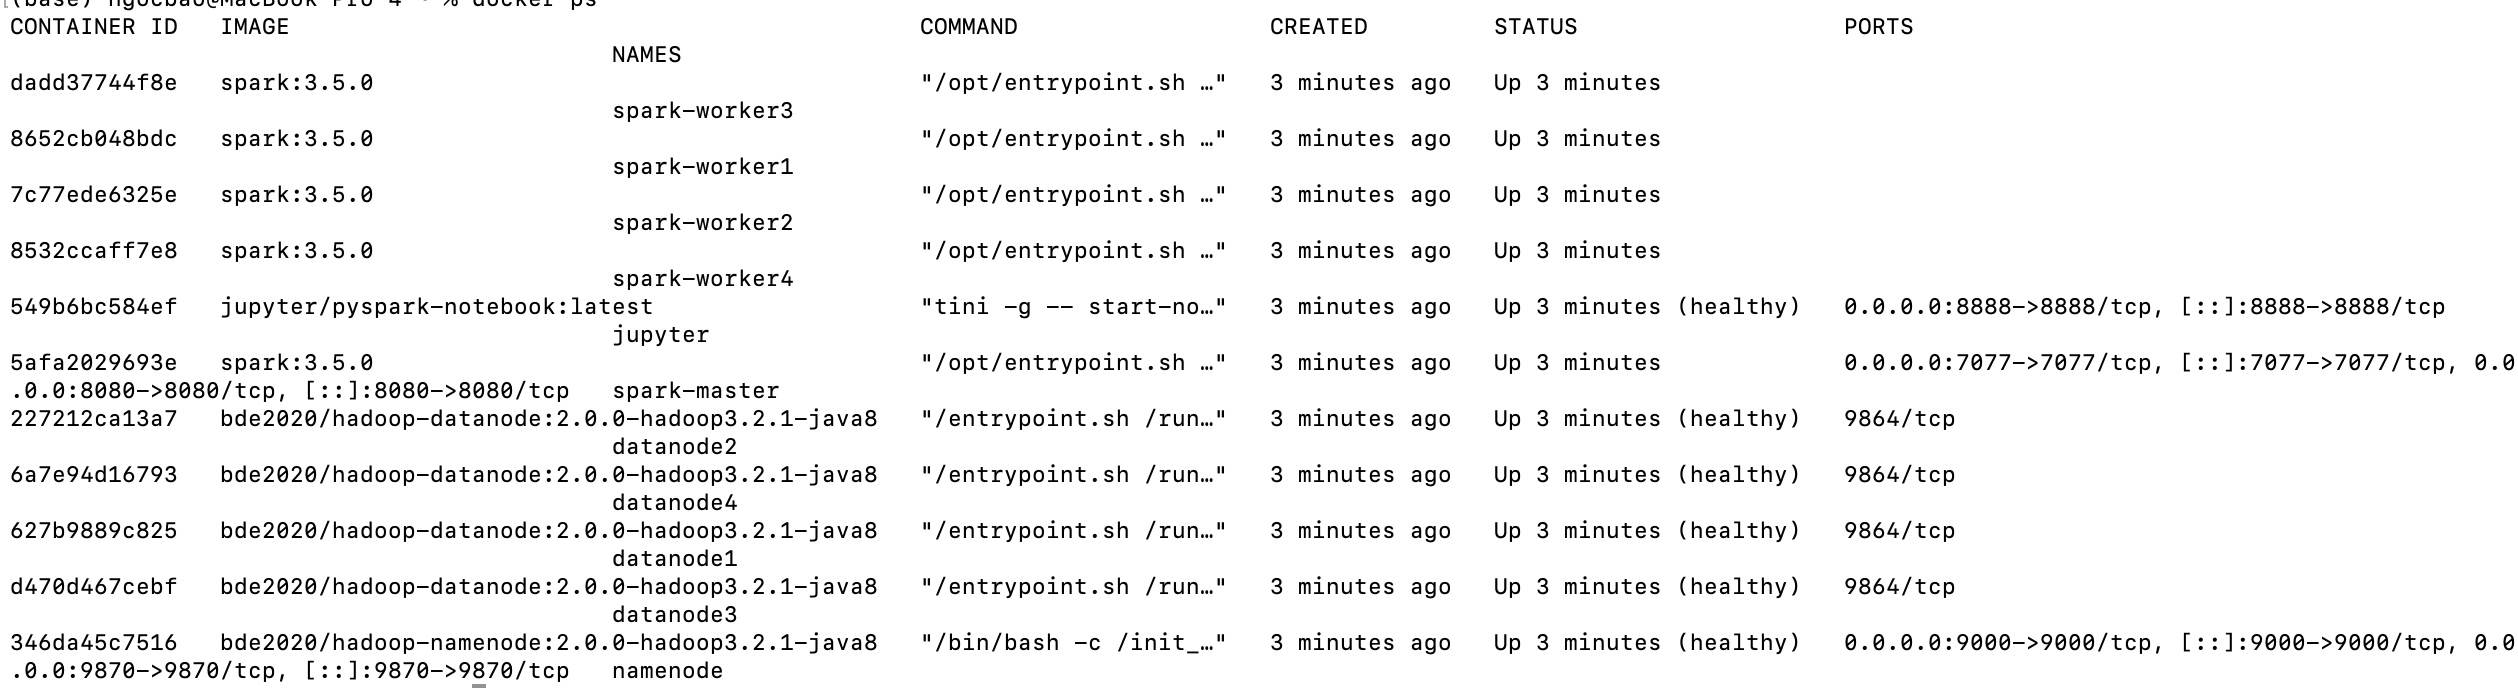
\includegraphics[width=0.9\textwidth]{virtual_cluster.png}
    \caption{Docker containers running in the virtual Big Data cluster.}
\end{figure}

This setup allows distributed processing and scalability across multiple nodes in a controlled environment.

\subsection{Connecting to the Spark Cluster}
We connect and create a Spark application using the kernel token displayed in the Jupyter log.  
Once connected, the Spark UI confirms active workers and job execution, as shown in Figure~\ref{fig:sparkui}.

\begin{figure}[H]
    \centering
    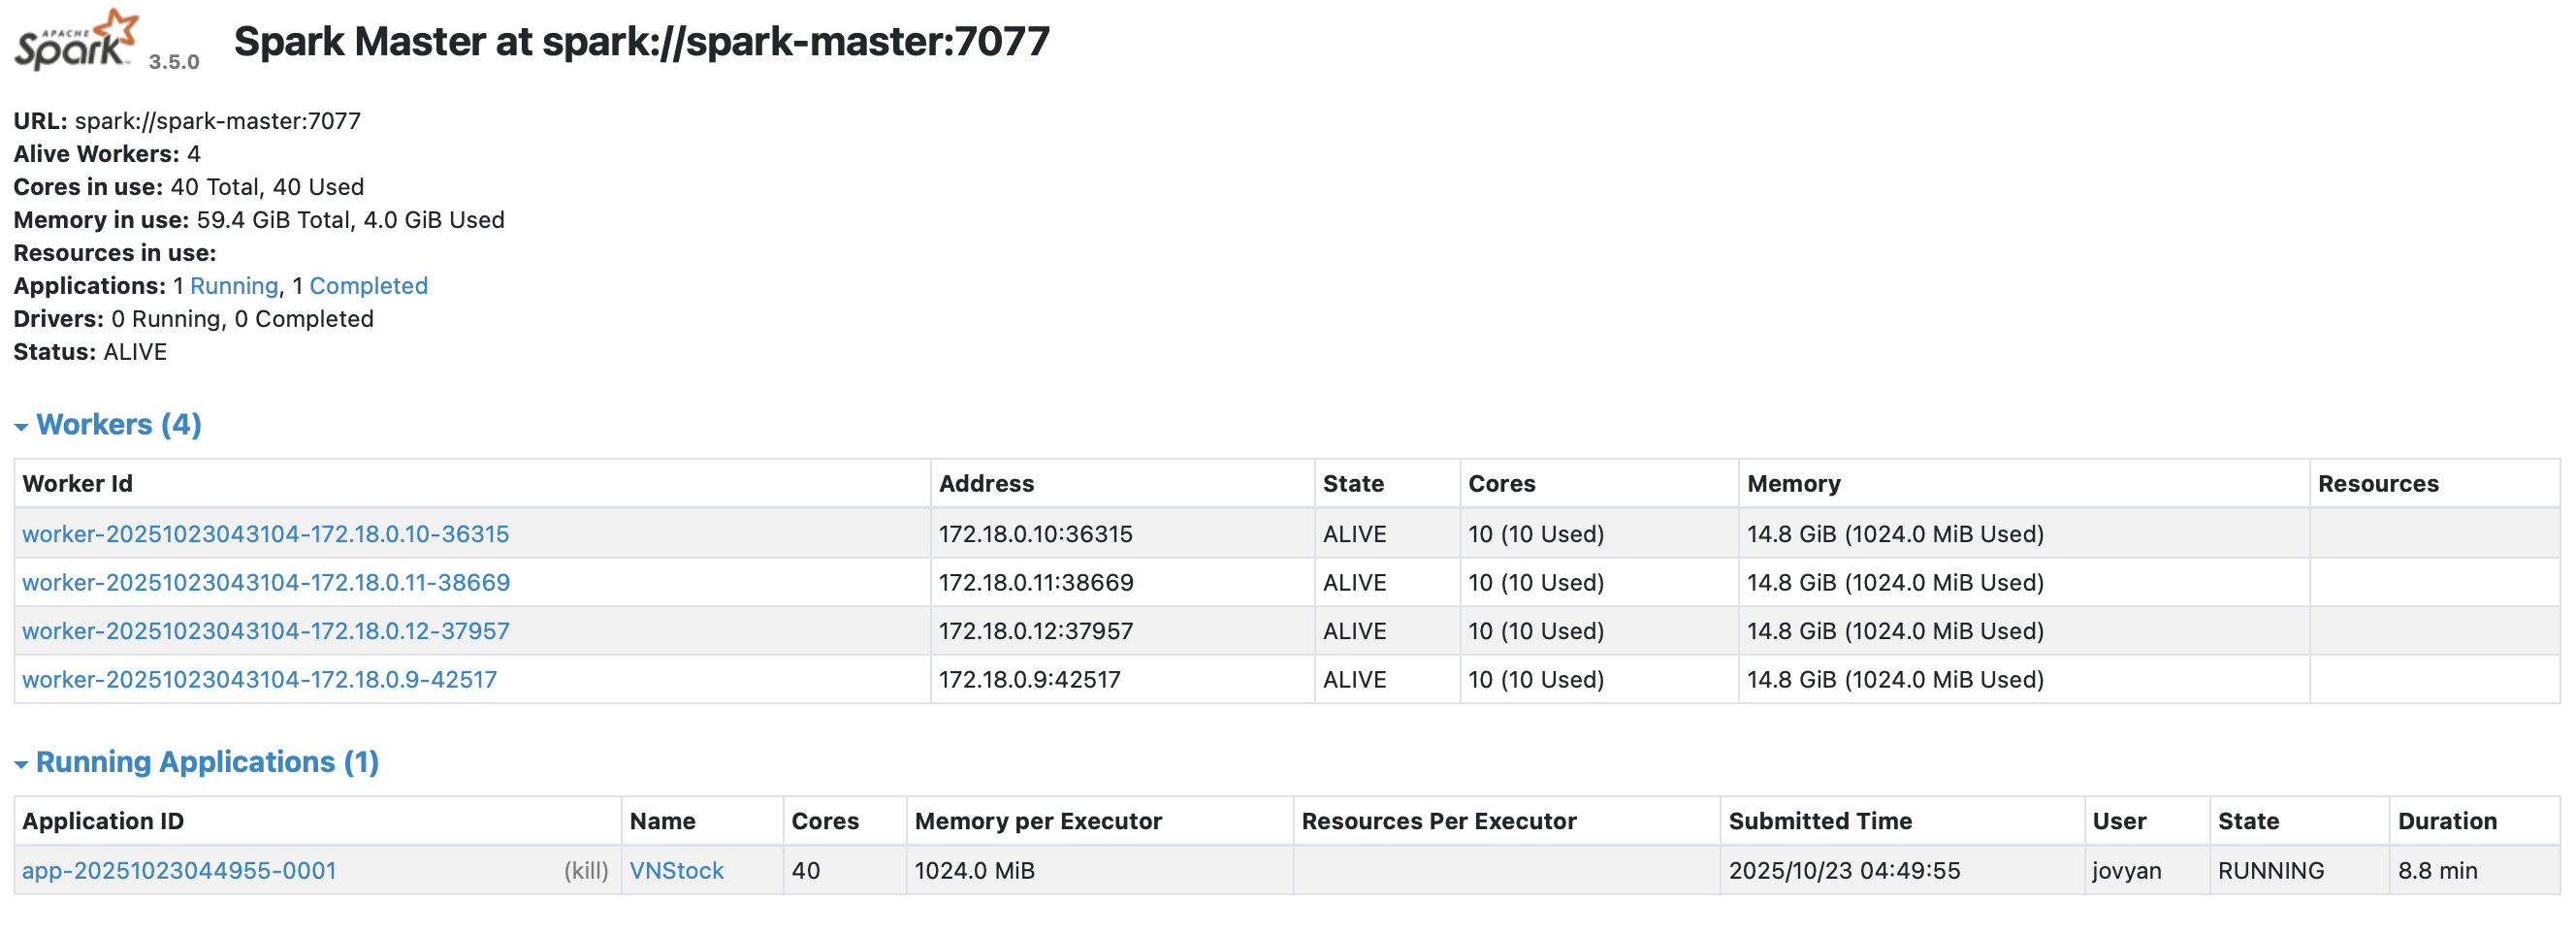
\includegraphics[width=0.9\textwidth]{spark_worker.png}
    \caption{Spark UI confirming successful cluster connection.}
    \label{fig:sparkui}
\end{figure}

%------------------- DATA COLLECTION -------------------%
\section{Data Collection}

The dataset consists of daily stock prices collected from VNStock for 10 major banks:

\begin{center}
\textbf{VCB, BID, CTG, TCB, MBB, ACB, VPB, HDB, STB, SHB}
\end{center}

\begin{table}[H]
\centering
\caption{Sample Trading Data of MBB (2015)}
\begin{tabular}{lccccc}
\toprule
\textbf{time} & \textbf{open} & \textbf{high} & \textbf{low} & \textbf{close} & \textbf{volume} \\
\midrule
2015-01-05 & 2.31 & 2.31 & 2.29 & 2.29 & 338{,}650 \\
2015-01-06 & 2.29 & 2.38 & 2.29 & 2.36 & 2{,}865{,}710 \\
2015-01-07 & 2.38 & 2.43 & 2.36 & 2.38 & 2{,}235{,}000 \\
2015-01-08 & 2.38 & 2.43 & 2.38 & 2.40 & 853{,}040 \\
2015-01-09 & 2.40 & 2.54 & 2.40 & 2.52 & 6{,}690{,}100 \\
\bottomrule
\end{tabular}
\end{table}

The dataset includes fields such as \textit{time, open, high, low, close, volume}, spanning the period from 2015 to 2025.  
Each stock’s data was saved as a CSV file and uploaded to HDFS for distributed analysis.

%------------------- PREPROCESSING -------------------%
\section{Data Preprocessing}

Before analysis, the data underwent several cleaning and transformation steps:

\begin{itemize}
    \item Converted date strings into \texttt{datetime} format.
    \item Removed missing or invalid records.
    \item Normalized stock symbols and price columns.
    \item Filtered the dataset to focus on the banking sector for consistent comparison.
\end{itemize}

These preprocessing steps ensure data consistency and reliability before Spark-based processing.

%------------------- DATA ANALYSIS -------------------%
\section{Data Analysis}

\subsection{Price Trend Analysis}
The closing price trend for each bank was analyzed to visualize performance over time.  
Figure~\ref{fig:trend} illustrates how selected banking stocks evolved between 2015 and 2025.

\begin{figure}[H]
    \centering
    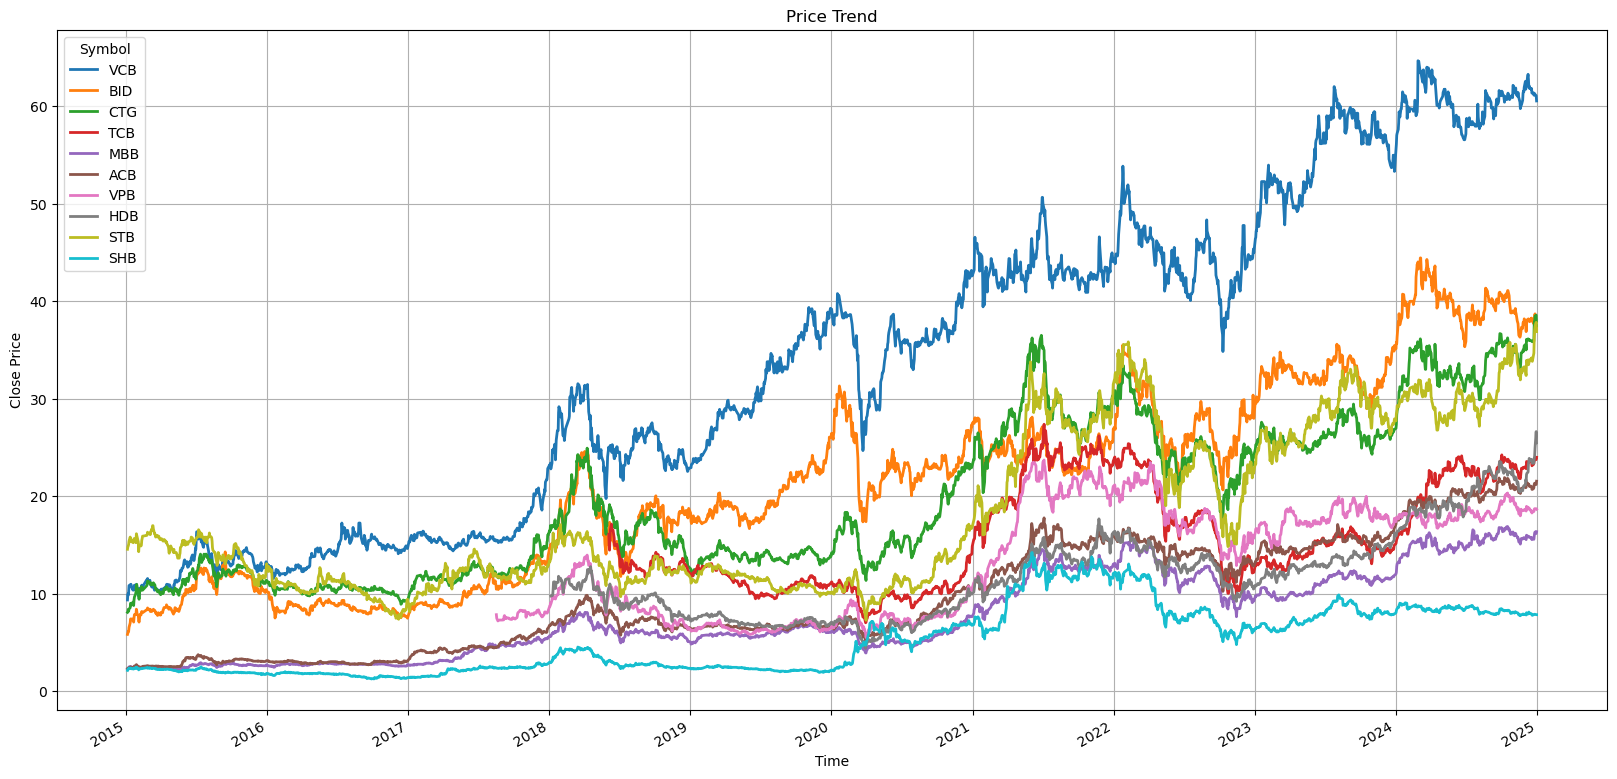
\includegraphics[width=0.9\textwidth]{price_trend.png}
    \caption{Price trends of major Vietnamese bank stocks (2015–2025).}
    \label{fig:trend}
\end{figure}

\textbf{Discussion:}  
The analysis reveals that most major bank stocks — particularly VCB and BID — experienced steady long-term growth despite short-term market corrections.  
Stocks such as MBB and ACB demonstrated strong resilience and long-term stability, reflecting solid fundamentals and investor confidence.

\subsection{Price Growth Rate Analysis}
The two-month price growth rate was computed to evaluate short-term and medium-term volatility among different bank stocks.

\begin{figure}[H]
    \centering
    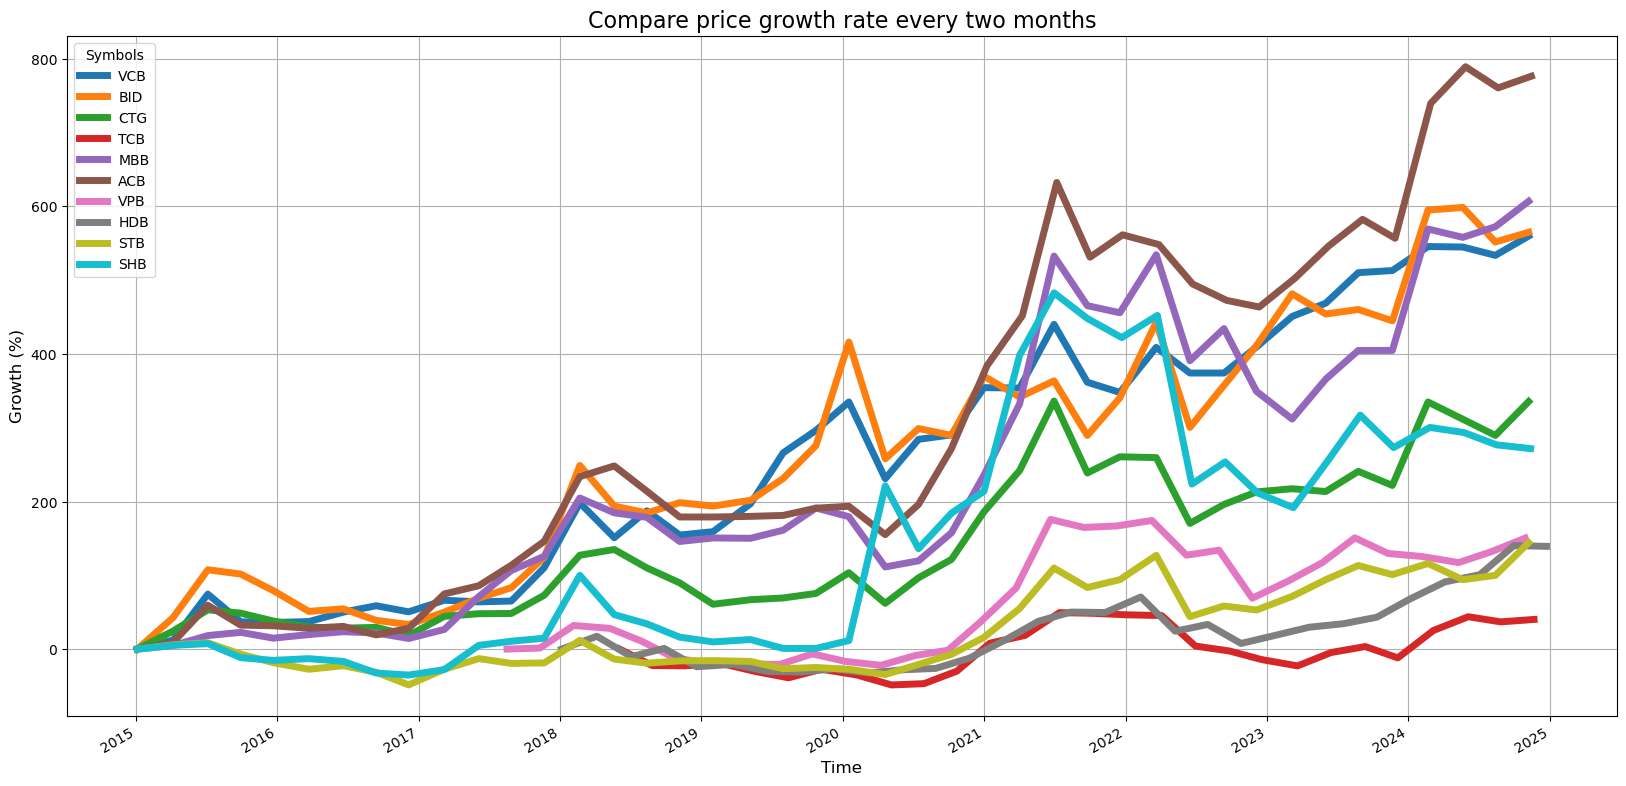
\includegraphics[width=0.9\textwidth]{price_growth_rate.png}
    \caption{Two-month price growth rate comparison among bank stocks.}
    \label{fig:growth}
\end{figure}

\textbf{Discussion:}  
The growth rate analysis highlights varying levels of volatility.  
Stocks such as ACB and MBB demonstrate higher fluctuations, implying higher risk but also potential for speculative gains.  
Conversely, BID and VCB maintain smoother growth trajectories, suggesting stable long-term investment opportunities.  
These insights can guide investors based on their risk tolerance and return expectations.

%------------------- PREDICTION -------------------%
\section{Prediction}

In this section, we present the results of stock price prediction for MBB and other major Vietnamese banks.  
The prediction model is based on a \textbf{Long Short-Term Memory (LSTM)} neural network trained on historical OHLCV data from 2015 to 2025.  
Data were normalized, sequenced with a 60-day lookback window, and used to predict the next day's closing price.

\begin{figure}[H]
\centering
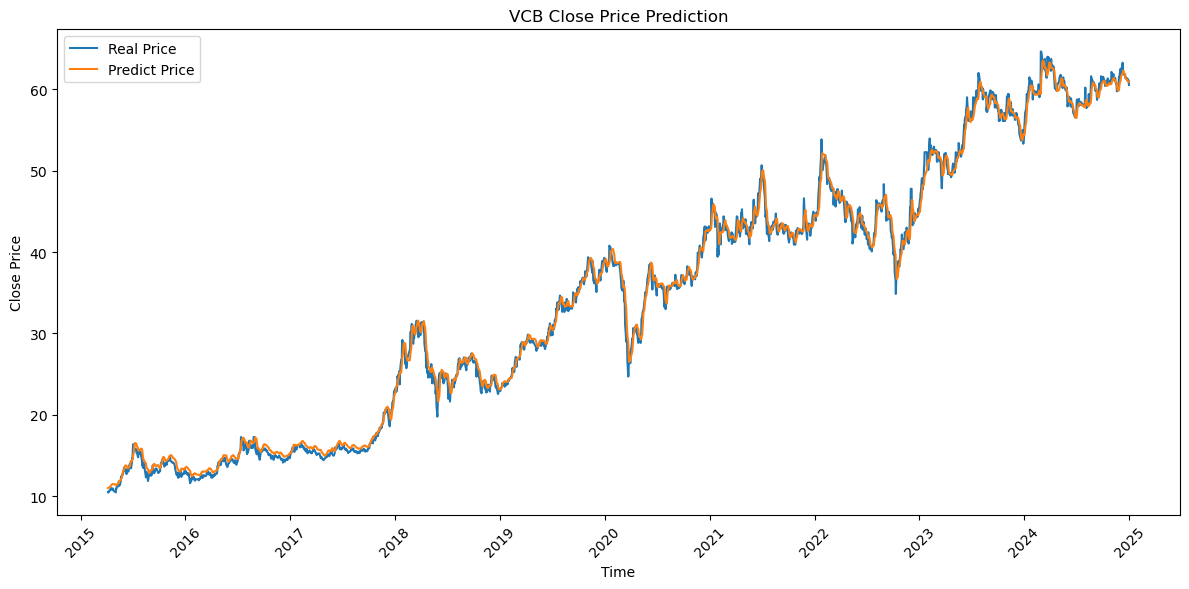
\includegraphics[width=0.75\textwidth]{prediction.png}
\caption{Actual vs Predicted Closing Prices for MBB (LSTM Model).}
\label{fig:prediction}
\end{figure}

The model achieves an $R^2$ score of 0.9968, indicating a strong correlation between predicted and actual prices.

%------------------- CONCLUSION -------------------%
\section{Conclusion}

This report presents the design and implementation of a Big Data analytics system for analyzing VNStock data using Hadoop and Spark.  
The system demonstrates efficient data collection, preprocessing, and distributed computation capabilities.  

Through analyses of price trends and growth rates, the study identifies differences in market behavior among leading Vietnamese banks.  
The results confirm that distributed Big Data technologies are effective tools for large-scale financial analytics and can provide valuable insights for both investors and researchers.

\vspace{1cm}
\noindent\textbf{GitHub:} \url{https://github.com/ngocbao220/Bigdata-ASM1-StockPrice}

\end{document}
